%\documentclass[a4paper, 11pt, titlepage]{article}
\documentclass{article}
\usepackage{a4wide}
\usepackage{amsmath}

\usepackage[pdftex]{graphicx}
\usepackage{pdfpages}
\usepackage{subcaption}
\usepackage{listings}
\usepackage{color}
\usepackage{cite}
\usepackage{import}
\usepackage[title,titletoc,toc]{appendix}

\usepackage{titlesec}
\usepackage{hyperref}

\setlength{\parindent}{0em}
\setlength{\parskip}{1em}
\renewcommand{\baselinestretch}{1.2}

\newcommand{\HRule}{\rule{\linewidth}{0.5mm}}

%Colours!
%\usepackage[table]{xcolor}
\definecolor{mygreen}{rgb}{0,0.6,0}
\definecolor{mygray}{rgb}{0.5,0.5,0.5}
\definecolor{mymauve}{rgb}{0.58,0,0.82}
\definecolor{mynavyblue}{HTML}{1E5A9C}

%PDF hyperlinks
\hypersetup{
     colorlinks   = true,
     citecolor    = black,
     linkcolor    = black,
     urlcolor   = mynavyblue,
     bookmarksopen  = false,
     pdfpagemode  = UseNone,
     pdftitle   = {Hexacopter Project 2015},
     pdfauthor    = {},
     pdfsubject = {Hexacopter FYP 2015}
}



%get a fourth section level by butchering the subsubsubsection command

\titleclass{\subsubsubsection}{straight}[\subsection]

\newcounter{subsubsubsection}[subsubsection]
\renewcommand\thesubsubsubsection{\thesubsubsection.\arabic{subsubsubsection}}
\renewcommand\theparagraph{\thesubsubsubsection.\arabic{paragraph}} % optional; useful if paragraphs are to be numbered

\titleformat{\subsubsubsection}
  {\normalfont\normalsize\bfseries}{\thesubsubsubsection}{1em}{}
\titlespacing*{\subsubsubsection}
{0pt}{3.25ex plus 1ex minus .2ex}{1.5ex plus .2ex}

\makeatletter
\renewcommand\paragraph{\@startsection{paragraph}{5}{\z@}%
  {3.25ex \@plus1ex \@minus.2ex}%
  {-1em}%
  {\normalfont\normalsize\bfseries}}
\renewcommand\subparagraph{\@startsection{subparagraph}{6}{\parindent}%
  {3.25ex \@plus1ex \@minus .2ex}%
  {-1em}%
  {\normalfont\normalsize\bfseries}}
\def\toclevel@subsubsubsection{4}
\def\toclevel@paragraph{5}
\def\toclevel@paragraph{6}
\def\l@subsubsubsection{\@dottedtocline{4}{7em}{4em}}
\def\l@paragraph{\@dottedtocline{5}{10em}{5em}}
\def\l@subparagraph{\@dottedtocline{6}{14em}{6em}}
\makeatother

\setcounter{secnumdepth}{4}
\setcounter{tocdepth}{4}





%unused refs
%OptoFlowStab


\begin{document}


  
\begin{titlepage}
\begin{center}

% Upper part of the page. The '~' is needed because \\
% only works if a paragraph has started.

\includegraphics[width=0.7\textwidth]{./logo.png}~\\[1cm]

\textsc{\Large Final Year Project Proposal}\\[0.5cm]

% Title
\HRule \\[0.4cm]
{ \huge \bfseries Towards Autonomous Search and Discovery in UAVs \\[0.4cm] }

\HRule \\[1.5cm]

% Author and supervisor
\noindent
\begin{minipage}[t]{0.4\textwidth}
\begin{flushleft} \large
\emph{Author:}\\
Brett \textsc{Downing}
\end{flushleft}
\end{minipage}%
\begin{minipage}[t]{0.4\textwidth}
\begin{flushright} \large
\emph{Supervisors:} \\
Prof.~Thomas \textsc{Braunl}\\
Chris \textsc{Croft}
\end{flushright}
\end{minipage}

\vfill

% Bottom of the page
{\large \today}

\end{center}
\end{titlepage}

  %\maketitle
  \begin{abstract}
  Multirotors are here to stay, and may soon be expected to interact in a human environment.
  Commodity quadcopters are advertising capabilities to act as  chase-cams and turn-key mapping solutions, but none of the current generation commodity uav chase-cams offer computer vision driven or even assisted flight modes to improve tracking, image framing or obstacle avoidance.  Such vision assisted routines would also apply to autonomous or semi-autonomous inspection tasks for fixtures in remote or hazardous environments.

  In this project, we re-designed and re-built the hexacopter platform inherited from previous year groups and implemented turn-key waypoint navigation and failsafe methods using the Ardupilot software stack.
  Using this platform, we developed and tested computer vision driven object tracking and navigation routines using limited computational resources. The aim  being to integrate vision assisted behaviours into future low-cost, lightweight UAVs.
  \end{abstract}
  \pagebreak
  \tableofcontents
  \pagebreak
  \section{Introduction}
  %aims
    PENDING THE APPLICATION OF SENSE
    
    %XXX Background, Aims
    %route map for project
    Recent Developments in power and control electronics has allowed small, consumer level UAVs to lift enough processing capacity to navigate at least partly by computer vision.

    %XXX

    We have developed computer vision driven chase cam processes for the 
     capabilities for a commodity multirotor UAV to act as a 
     the remote object informed by computer vision alone.

    In order to keep a well rounded perspective on our scope, the team agreed to design set our respective scopes as interdependent modular components in a much larger system.  This made it painfully clear when the scope or generality of our work fell short.
    Tan \cite{Tan} developed a library of feature detection and extraction routines and assessed the optimisation potential for each on the single board computer of our platform.
    Allen \cite{Allen} investigated means of implementing collision avoidance on a UAV, developing a robust algorithm to find the shortest detour around an exclusion zone, and experimenting with low-confidence occupancy grids.
    Mohanty \cite{Mohanty} worked on Capture and Tagging of images to suit proprietary offline 3D reconstruction algorithms, and the generation of paths with which to scan objects and fields.

    The Computer vision driven chase-cam behaviour described here is based on the optimised Computer Vision routines under active development by Tan \cite{Tan}.

    All Motion Control routines in the code base were designed keeping in mind that they must eventually be integrated with the collision avoidance and geo-fencing routines developed by Allen \cite{Allen}.  This included the mapping paths used by Mohanty \cite{Mohanty}.

    Development of the object tracker placed a strong focus on the capabilities of the platform.  We saw fit to undertake a critical review of all aspects of the platform, and make improvements that facilitate the current typical feature set.

    The inherited platform did not meet our requirements

    We have developed a suite of computer vision processes to detect and locate features in the camera frame,  objects, compute 

    and proven them as GPS-assisted control routines.

    %route map for report
    Object tracker and Platform discussed in two separate sections.


  \section{Background}


    %XXX unapologetically copied from proposal doc, needs updating and expanding
    \subsection{Motivation}

      A number of Commercial Micro UAVs are beginning to advertise the ability to act as an autonomous chase-cam \cite{Lily} \cite{AirDog}.  Almost all of these systems rely on a tracking device on the user, and many navigate entirely by GPS.  While the performance of GPS is improving, the performance of a chase-cam will be limited to the update rate and fix accuracy of the beacon and drone GPS modules.  It also requires a GPS lock and radio link to be achieved and maintained in both devices for the system to function at all.

      The power distribution and plant monitoring sectors have recently been taking on small fleets of drones to perform routine inspection of remote, hazardous or otherwise difficult locations \cite{RopeAccess}.  Many of the tasks are reasonably repetitive and well defined enough to fully automate, but cannot be navigated by GPS alone due to the poor repeatability resulting from GPS signal drift.
      During this project, we were approached by a mining safety startup interested in using UAVs for routine site inspections.

      The UAVs we are targeting operate with small payloads, must react quickly to changes in the environment, and frequently feature camera systems.
      Despite falling costs of hobby and toy grade multirotor systems, Collision avoidance, Object tracking, mapping and inspection are not well catered for in the current UAV market.
      Very few sensors are of the appropriate scale, or mass for low cost UAVs.
      Ground based vehicles have an advantage in that a 1D sensor need only be swept in one axis to search for obstacles, whereas a UAV must collect data filling a volume ahead of it. About the only form of sensor capable of doing this is a 3D laser scanner which is a high-precision, high-cost, high-mass device.
      A simple camera collects data on at least two axes at high enough speeds to navigate a multirotor, but the data is often difficult or computationally expensive to interpret.

      With environmental data collected by an efficient computer-vision routine, the current generation of multi-rotor devices would be able to interact with a human environment.

      Computer Vision assisted control routines would permit common low cost UAVs to better frame extreme sport chase-cam film reels, automatically avoid obstacles, and stabilise GPS variances in remotely operated inspection tasks.

      In this study we investigate the usability of computer vision alone to track and follow a moving target.  It is hoped that this work can be used to improve the performance of camera tracking routines in autonomous chase-cam and cinematographic applications, and partially automate remote inspection applications.

      Much of the technology related to multi-copters is applicable to most other forms of UAV.  The vast array of tasks micro UAVs have already been applied to suggests our work may find use in Agriculture, mapping, targeted crop dusting, Cinematography, extreme-sport photography, Data collection, remote observation and inspection, and hazard and environmental monitoring.
        %Check the grammar here
    \subsection{Related Work}
      \subsubsection{Optical Search}
        Search and Rescue lend themselves to automation due to the difficulty in mobilising teams in remote, harsh or dangerous conditions.  A micro UAV can be deployed quickly and commence the search operation before boots can be placed on the ground.
        The UAV Outback Challenge \cite{OutbackChallenge} is a regular competition to perform various search and rescue missions.  The performance demands are deliberately set very high, and the competition frequently goes uncompleted.  
        In 2012 CanberraUAV \cite{canberrauav}, a UAV development team from Canberra completed the search aspect of the competition.
        After trying a number of image recognition algorithms, the search algorithm that they flew with simply looked for the blue of the jeans of Outback Joe \cite{tridge}. This was sufficient to locate the target in a 4x6 km area.  This goes to show that even a minimally complex routine can be effectively applied in appropriate conditions.

      \subsubsection{Terrain Estimation via Optical Flow Methods}
        Adding sensors to allow the copter to understand its environment is a surprisingly difficult task.  Conventional contact methods operate at ranges far too close for UAVs. Ultrasonics are buffeted by down-wash and most depth sensors are either too heavy or suffer under intense light.
        In terms of simplicity of algorithms, biomimicry has turned up some surprising results.  In 2004, a French research group applied a number of optical flow algorithms inspired by insect vision to the navigation of a small helicopter \cite{InsectFlowMethods}.  The computer vision routines were used to inform the navigation loops, following the middle of urban tunnels and reducing speed in dense clutter, without necessarily computing the distance to the obstacles.  These routines were relatively expensive in terms of computational power, but extremely simple and parallelizeable.

      \subsubsection{Position Estimation using Stereoscopic Methods}
        Any measurement will have an associated uncertainty. Extracting the most information out of a collection of measurements rarely requires taking the most accurate measurements.  It is possible to estimate the position of an object or feature using multiple images separated in either space or time, but making effective use of the information requires an understanding of how the uncertainties behave.  Error Modelling in Stereo Navigation \cite{stereoUnc} utilizes a number of routines to estimate the position of a vehicle by tracking visible land-marks in a stereoscopic system; and notes the interaction between the geometry of the uncertainties, and the stability of the result.

      \subsubsection{Altitude Estimation and Odometry by optical flow}
        Elementary methods are still interesting for the sake of biomimicry.  A 20 element photo-array was demonstrated to provide sufficient resolution to control the altitude of an aircraft \cite{optoAlt}, coupling the altitude to the velocity.
        Dedicated, low resolution optical flow sensors have become exceedingly cheap since the market-saturation of the optical mouse; and many commodity flight computers already include doppler information from GPS modules. 
        Combining these elements allows a UAV to estimate the distance to the terrain, \cite{RemTerrain}.  These commodity sensors typically do not include circuitry for computing rotation, but given the cost of the sensors, that limitation can be overcome combining two sensors \cite{FlowRot}.
        A number of UAV systems such as ArduPilot already include support for these devices in their code-base \cite{ArduFlow}.
        This support also covers pitch and roll compensation and position stabilisation using optical odometry.

      %\subsubsection{Uncertain Geometry}

    \subsection{Project History}

      \subsubsection{2013}
        The 2013 team of O'Connor \cite{OConnor} and Venables \cite{Venables} established the UAV research project with the purchase of a DJI ``flame-wheel'' F550 Hexacopter with a NAZA-lite flight controller.  This copter was fitted and tested, and finally converted into an autonomous platform with the addition of a Raspberry Pi single-board computer (RPi) and a circuit to switch the control channels from the radio receiver to the RPi GPIO outputs.
        The NAZA-lite at this time did not feature telemetry outputs or way-point inputs, but it was able to loiter in a stiff wind using a GPS fix.
        This team gathered location information for the RPi using a Qstarz GPS unit, and bearing information using an X-sens IMU.  The weight of the sensor duplication did not exceed the maximum payload capacity of the platform, but it did compromise flight-time.
        Under direct control from the RPi, the drone was able to execute basic way-point navigation.
      \subsubsection{2014}

        The 2014 team of Baxter \cite{Baxter}, Mazur \cite{Mazur} and Targhagh \cite{Targhagh} added an internet accessible web UI to control the various autonomous features of the original platform, displaying the flight-path of the copter and a live feed from the camera.
        The navigation routines were improved and extended to permit operation in the absence of reliable heading information, and the computer vision routines were extended.

  \section{Platform}
  %describe the hardware in detail.
    \subsection{Introduction}
      %introduce why you are focussing on the platform.
      %reset image.
      At initial handover, 

Control Handover
Sensor Duplication
New Flight Controller
Telemetry
Simulation Environment
Web UI

      We reviewed the previous team's hardware configuration and prepared a report outlining the weaknesses and proposing a new approach.
    
      The flight hardware is a major component of the control loops in the object tracker, and the performance of these loops cannot be ignored.
      For a multi-copter to move forward, it must control the speed of the props to create a pitch angular acceleration. The pitch angle is stabilised to generate a forward acceleration which is used to control position.
      Contrast this with a ground based robot where the navigation routines interact with a mechanically well-constrained system.
      
      At almost every stage of this fifth order dynamic system, the flight mechanics introduce perturbations to any additional control system with a particular intent.

      In order to support the object tracker, the platform must meet certain minimum requirements in both performance and telemetry.


    \subsection{Architecture and Methodology}
      %>minimum requirements
      %>theory of the requirements of the platform
      %>describe the control architecture required for the object tracker
      %>Preferable Architecture

      This project centred around a hexacopter based on the DJI F550 ``Flame Wheel'' frame. This frame allows for a generous lift capacity, and plenty of space to fasten flight assist hardware, and represents a low cost platform so that our work can be reproduced by a sufficiently motivated hobbyist.

      %XXXFlight controller
      In this work, the flight tasks are based around two physically separate processors; the Flight Controller, and the Server. This allows a stable, known-safe build to be maintained on the flight controller, while experimental code runs on the server. If the server fails for any reason, the flight controller will maintain flight, and it allows the operator to engage various fail-safe behaviours without having to rely on the experimental code.
      
      At initial hand-over, the fight controller was a DJI NAZA lite.
      
      %XXXprocessor, gimbal
       server was a Raspberry Pi model B+, and

      %>objective of the platform (with history)
      The NAZA and RC emulation for autonomous flight did not fit together well. The NAZA lite is designed as an entry level free-flight controller and does not expose any interfaces for telemetry or data acquisition.  As a result, the previous teams had to duplicate the GPS and IMU sensors to make such information available to the server's algorithms.

      The NAZA Lite also does not feature waypoint navigation features, or secondary command channels so the previous teams used a relay board to physically switch the control inputs from the RC receiver to the server, and implemented their own flight control algorithms on the server.
      This breaks the assumption that the flight controller will maintain flight during a server crash.  Indeed, we were told that server lock-ups frequently caused the craft to power-dive.

      %>critical review

      %The copter now boasts a very complete feature set 


    

      %>how to test for compliance min performance criteria
      


  \subsection{Results and Dicussion}
    %(fitness for purpose etc)

    The server has been upgraded to a Raspberry Pi V2 single board computer, which we still regard as a computationally starved platform.  At the time of writing, the Raspberry Pi V2 has less computational power than a smartphone in the \$200 price bracket.
    \subsubsection{Control Handover}
      The physical switch of control from the user to the server, and the ongoing development of a control loop meant that RC switch was never configured to surrender the throttle channel, and the server was left without altitude control.  This meant that the server had continuous perturbations from the user who remained responsible for maintaining a fixed altitude by sight alone.


    \subsubsection{Sensor Duplication}

      %XXX(image: GPS track, glitch from Uni Club to Eng Carpark)

      We made some attempts to break into the data channel between the NAZA flight controller and its GPS module, but the raw GPS and compass data was not particularly useful without the accelerometer and gyro data.  This channel had also been deliberately obfuscated by DJI, making it quite clear that this was beyond the design intent of the flight controller.  A community RC group had reverse engineered this link, and we ported their code to the raspberry pi and removed the Qstar-z GPS unit.
      
      %XXX How many commas do you want!?
      The new configuration allowed us to fully eliminate duplicated hardware, an opportunity to fully re-build the wiring harness, and significantly reduce the weight of the craft, extending the flight time to almost twenty minutes.
      Near the end of the project, we fitted a second GPS module to the copter to combat the poor multipath environment of the UWA campus.  With the sensor fusion and Extended Kalman Filter in the Ardupilot firmware, we we able to fly on GPS alone in some of the worst urban canyons in the campus.


      The server did not have access to an estimate of remaining flight time, and the user could not retrieve logs in the event of a crash.

      Waypoints were handled on the server despite the NAZA featuring GPS assisted loiter behaviour, and a reliable return-to-launch failsafe feature.  In general, control loops should be as short as possible, and routing them through an entirely separate processor is clearly suboptimal.
%an unnecessarily long loop
    \subsubsection{New Flight Controller}
      We swapped the NAZA flight controller out for a 3DR Pixhawk running the Ardupilot 3.3 firmware.  This gave us Waypoints, altitude control, failsafes, telemetry, and a GPS-only driven follow-me mode out of the box.
      The open and configurable flight controller with built-in autonomous and hybrid modes allowed us to fully surrender control to the autonomous platform, including altitude control.  The built-in mode change behaviours meant that we could relinquish and resume manual control at the remote, or activate fail-safes just as reliably as with the NAZA.
      
    \subsubsection{Telemetry}
      The telemetry link supports the MAVlink protocol, which defines various commands from interrogating the status to setting waypoints, or even setting the instantaneous velocity vector.
      This let us keep the high-speed components of the control loops firmly inside the flight controller, and direct it with the lower speed vision tasks.  This also gave us linear control inputs in SI units.

    \subsubsection{Simulation Environment}
      By using a fully-featured open-source flight controller, we also had access to the community developed simulation environment.  
      The Ardupilot simulator is designed to simulate the behaviour of the flight controller against various hardware configurations and flight styles.  As such, it incorporates a comprehensive inertial model and noise injection to the various sensors.
      We were able to compile our tests for our development machines couple them to the simulator over a local TCP socket, and test them against the same version of the flight control firmware as we had uploaded to the physical copter.


    \subsubsection{Web UI}
      We saw fit to refresh the Web UI and HUD, implementing a more appealing and maintainable template system, and adding more information to the display.
      The Web UI works on almost all devices.

\section{Object tracker}
  \subsection{Introduction}
  
    Tracking objects requires a long chain of systems to work in unison.  From tracking features in single images, all the way to reconstructing and navigating the environment without losing sight of the object.
    By focussing on extreme sport cinematography as the end goal of the project, the bar was set deliberately high.
    Tracking high-speed, high-acceleration objects requires a large control bandwidth and accurate compensation for perturbations injected by the flight hardware.  

    At hand-over, the platform contained a chase-cam algorithm that used a PID loop between the position of the object in the image frame and the RC inputs to the flight computer.  Venables \cite{Venables} notes that the system does not deal well with changes in altitude, or perturbations in pitch and roll.  We found it was not able to follow a high contrast marker under modest accelerations in most conditions.

    We have broken the process into clearly defined estimation steps to expose implicit assumptions, and incorporated some features from modern SLAM processes.  Our have efforts resulted in an end-to-end chain of modular software, with some functions migrated onto the flight controller to shorten control loops and enhance stability. 

  \subsection{Method}

    \subsubsection{Position estimation}
      %XXX existing or new PID system, make it clear that that changed
      After experimenting briefly with the existing PID loop process, we moved on to basic triangulation methods to estimate the location of an object with the assumption that it was on the ground.  We estimated the height based on the GPS altitude data streaming from the NAZA GPS; but without access to the NAZA's internal barometer, the uncertainty in height caused the navigation loop stability to vary significantly minute by minute.
      After upgrading to the Pixhawk, we had access to the data from the Extended Kalman Filter in the flight controller.  We also made significant changes to the way the flight controller was guided by the server, and this prompted a near total re-write of the object tracking code-base.

    \subsubsection{Desired relative pose}
      Once the object is located in 3D space, the copter will calculate a vantage point from which to view it.
      This vantage point could include information regarding the terrain, the size and trajectory of the object, the field of view of the camera, locations of light sources etc.  This is the point at which cinematographic style is included in the chain.

      The camera position used in testing selects the nearest point at the copter's current altitude, on a cone of a given slope radiating upwards from the object.
      The uncertainty analysis (discussed in section \ref{sec:UncertaintyAnalysis}) is available to this algorithm, and could be used in a SLAM system to select a pose that will most efficiently reduce the uncertainty of a given landmark's location.  Computation of uncertainty-minimising poses can lend an observation priority metric to systems such as those used in cooperative robotics \cite{TrilatUnderwater}.

    \subsubsection{Motion Control}
      As of version 3.3, The Arducopter code-base has support for arbitrary velocity vectors.  The first iteration of the motion control algorithm mirrored the old RC emulation code base and transmitted a velocity vector in body coordinates to the flight controller and closed the motion loop through the automation server.  The long feedback loops had problems with delays and required detailed tuning.
      The Pixhawk already has advanced automatic tuning routines and performs very well as a standalone autonomous platform.
      To further reduce feature duplication, we replaced the motion control code with a guided-mode waypoint.  The automation server then simply computes and transmits the desired vantage points and yaw values to the Pixhawk.

      The coming Arducopter 3.4 release is set to include more advanced control schemes and support for GPS-independent autonomous features.  All of the motion control processes were kept in the code-base for comparisons and future work, particularly to facilitate a fully GPS-independent acceleration vector control scheme.

      The command structure on the Pixhawk supports dead-channel detection and can execute failsafe behaviours on loss of link.  Even if our motion control system were to use an Acceleration vector output, a loss of link or server crash would engage the appropriate fail-safe, and the copter would continue flying.

    \subsubsection{Structure from image}
      Resolving structure from image is a field unto itself.  In general, the computational load of modelling the environment in three dimensions live is beyond the capabilities of supercomputing clusters that would fit in the mass restrictions of most multi-rotors.  However, Simultaneous Localisation and Mapping (SLAM) systems optimise components of this field into a vast array of algorithms of varying computational power requirements.
      One of the critical features of modern SLAM systems is an acknowledgement that every measurement comes with some uncertainty. 
      The treatment of uncertainty can be very simple, carrying a one-dimensional confidence value; through to very complex, where every aspect of the measurement is recorded for post-processing where non-linear couplings can be accounted for.

      Some systems are beginning to feature graph-traversal techniques where observations are stored as relative links in a graph, and networks are drawn through those links to optimise against the uncertainty of various aspects of the environment.  These techniques allow the landmarks to be unloaded from memory very easily permitting a small live map, and can approach the detail of full-map covariance methods by using a less-than-live graph traversal process.

      %XXX get a reference
    \subsubsection{Observations and uncertainties}

    %Make it clear how much of this approach you developed yourself.
    %Maybe also mention your work in 'Related Work'
      \subsubsubsection{Observation to Object Allocation}
        \label{sec:objectAllocation}
        With many observations streaming from the camera simultaneously, the algorithm must decide which observation relates to which object in memory.

        We developed and tested several algorithms to differentiate objects and refine uncertainties.
        Most of these suffered from the objects' uncertainties falling so low that the probability of intersection between observation and model fell below reasonable thresholds and new object models were generated.  Part of the problem being that our object detection is still based on colour thresholding.  This generates objects of significant size.  Sized objects violate the assumption implicit in the normal distributions where the probability of locating an ``object'' at a zero sized point, is zero.

        In order to facilitate rapid testing and expose weaknesses, the algorithm we have field tested with deletes and regenerates the objects every cycle unless the object leaves the field of view.  This makes it very clear when the object estimation code is behaving erratically.
%XXX 
      \subsubsubsection{Uncertainty Analysis}
        \label{sec:UncertaintyAnalysis}

        A good uncertainty model encodes everything that is known and nothing of what is unknown.  Good treatment of uncertainties combines knowledge without losing information, or adding assumptions.
        In the case of structure from image, a system that extracts maximal information from a single camera should be automatically capable of full stereoscopy using only the uncertainty analyses that applied to the monocular case.
      

      \subsubsubsection{Ellipsoidal models with Covariance Matrices}
        For the sake of computational load, we've assumed the collected data has a three dimensional multivariate Normal distribution.  We use the quadratic form which uses the inverse of the covariance matrix.
        \begin{equation}
        PDF = \frac{1}{\sqrt {(2\pi)^k|\Sigma|}} e^{-\frac{1}{2}\left( \left(x-\mu\right)^T \Sigma^{-1} \left(x-\mu\right) \right)}
        \end{equation}
        where
        \begin{equation}
        \Sigma=\begin{bmatrix}
          \sigma_x^2 & \sigma_{xy} & \sigma_{xz} \\[0.3em]
          \sigma_{yx} & \sigma_y^2 & \sigma_{yz} \\[0.3em]
          \sigma_{zx} & \sigma_{zy} & \sigma_z^2 
        \end{bmatrix}, k=3
        \end{equation}
        %XXX get the justification for the product straight
        This form is particularly useful because the normal distribution behaves as a probability density function of prediction, and the combination of two observations is the normalised product of probability density functions.  The product of two elliptical Normal distributions is also an elliptical normal distribution.  
%XXX check all the tenses
        In order to save on computing resources, we use the inverse of the covariance matrix natively \(C\), and ignore the normalisation constant, which has a closed form solution and can be calculated from the inverse covariance matrix directly as follows:
        \begin{equation}
        \frac{\sqrt{|C|}}{\sqrt{(2\pi)^3}}
        \end{equation}
        This allows a slightly faster rasterisation of the probability density than covariance matrices, but more importantly, follows almost exactly the definition of an ellipsoid and permits highly efficient geometric manipulation:
        \begin{equation}
        1 = \left(x-x_0\right)^T A \left(x-x_0\right)
        \end{equation}

        With no normalisation constant, the distribution always has a value of exactly one at the centroid.
        By permitting singular matrices, the ellipsoidal format has the flexibility to represent uncertainty distributions unbounded in length in any direction, representing rays and planes.  Such distributions are extremely common as measurements, an absence of information about constraints along a given axis would just be a zero in he inverse covariance matrix \cite{UncertainGeo}.  These singular forms still combine efficiently to form non-singular localised distributions.
        
      \subsubsubsection{Combining measurements}
        The covariance structures are well suited to use as vectors, automatically calculating the uncertainty of any combination of vectors. 
        %XXX hacks and proofs should probably go to the appendices
        Multiple observations of a single point are generally combined with a weighted average, but assigning weights to superior measurements is often difficult as is a common point of discussion in Kalman Filter design.
        
        If the subject of the measurements is known to be the same object, the object is likely to be at the centroid of the product of the probability density functions.  This takes measurement accuracy into account.
        Using the form above, the product of density functions becomes the sum of polynomials.
        \begin{figure}
        \centering
        \begin{subfigure}{.3\textwidth}
          \centering
          
\includegraphics[width=.8\linewidth]{images/GaussianLine1.png}
          \caption{Measurement 1}
          \label{fig:uncProdsub1}
        \end{subfigure}%
        \begin{subfigure}{.3\textwidth}
          \centering
          
\includegraphics[width=.8\linewidth]{images/GaussianLine2.png}
          \caption{Measurement 2}
          \label{fig:uncProdsub2}
        \end{subfigure}
        \begin{subfigure}{.3\textwidth}
          \centering
          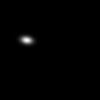
\includegraphics[width=.8\linewidth]{images/GaussianLine3.png}
          \caption{Combined Measurements}
          \label{fig:uncProdsub3}
        \end{subfigure}
        \caption{The Product of Two Measurement Ellipsoids}
        \label{fig:uncProd}
        \end{figure}

        \begin{equation}
        C_3 = C_1+C_2
        \end{equation}
        \begin{equation}
        \mu_3 = C_3^{-1} . (C_1.\mu_1 + C_2.\mu_2)
        \end{equation}
        Clearly apparent here, is that \(\mu_3\) is undefined if \(C_3\) is singular.
        This is not a loss of generality, merely an artefact of the matrix form.  If the matrix \(C_3\) represents a ray, \(C_3\) will have one eigenvalue of zero and \(\mu\) will have a degree of freedom along the corresponding eigenvector.
        
        This method minimises the sum of the squares of the Mahalanobis distances between the result and the initial two ellipsoids.  This property of minimised Mahalanobis distances is maintained with additional ellipsoids, effectively creating a least sum of squares regression method that accounts for the covariance geometry of each measurement as successive ellipsoids are added to the mix.
        This least squares regression method becomes obvious in the case of spherical distributions.  The successive combination of \(n\) measurements, each with an assumed variance of \(\sigma^2\), will have a resultant variance of \(\sigma^2/n\) which is consistent with treatment of uncertainties in the one dimensional case.

        In a network of observations, using this transformation destroys the assumption of independence of the observations.  A full covariance matrix method would track this by generating cross terms.  The Covariance Intersection described in \cite{CovarNoCorrel} provides a weighted method of fusing observational data while keeping the uncertainty estimate conservative enough to retain the assumption of independence.

      \subsubsubsection{Vector Transformations}
      
        \paragraph{Vector Sum}
          Treating the ellipsoids as approximate displacement vectors requires the definition of vector operators.
          Again, the matrix form below does not permit singular Matrices as inputs nor outputs, but unpacking it into polynomial form does allow suitable centroids to be chosen.
        \begin{figure}
        \centering
        \begin{subfigure}{.3\textwidth}
          \centering
          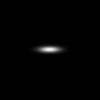
\includegraphics[width=.8\linewidth]{images/GaussianSum1.png}
          \caption{Object at the Origin}
          \label{fig:vectSumsub1}
        \end{subfigure}%
        \begin{subfigure}{.3\textwidth}
          \centering
          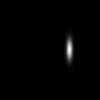
\includegraphics[width=.8\linewidth]{images/GaussianSum2.png}
          \caption{Uncertain Displacement}
          \label{fig:vectSumsub2}
        \end{subfigure}
        \begin{subfigure}{.3\textwidth}
          \centering
          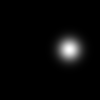
\includegraphics[width=.8\linewidth]{images/GaussianSum3.png}
          \caption{Final Object Location}
          \label{fig:vectSumsub3}
        \end{subfigure}
        \caption{The Vector Sum of Two Uncertainty Distributions}
        \label{fig:vectSum}
        \end{figure}
        \begin{equation}
        C_3 = (C_1^{-1} + C_2^{-1})^{-1}
        \end{equation}
        \begin{equation}
        \mu_3 = \mu_1 + \mu_2
        \end{equation}
        Again, this ignores cross terms that would be generated from a full covariance matrix.  It can be thought of as a means of collapsing multiple chained, relative observations or motion estimates into a single relative observation.

        \paragraph{Scale}
        \begin{equation}
        C' = S^{-2} C
        \end{equation}
        \begin{equation}
        \mu' = S \mu
        \end{equation}

        \begin{equation}
        S=\begin{bmatrix}
          S_x & 0 & 0 \\[0.3em]
          0 & S_y & 0 \\[0.3em]
          0 & 0 & S_z
        \end{bmatrix}
        \end{equation}
        Where \(S_n\) represent the change of scale along any axis.
        The scale operator can be used to reverse the direction of a vector.  This allows the definition of a discreet time derivative \(\dot{x} = (x(t_1) - x(t_2))/(t_2-t_1)\).  A positional derivative defined in this way has an appropriately large velocity uncertainty distribution that increases in size with shorter time-steps, but can be averaged by intersecting multiple samples of velocity.

        \paragraph{Rotate}
        The ellipsoidal structure can be rotated as follows:
        \begin{equation}
        C' = R^{-1} C R
        \end{equation}
        \begin{equation}
        \mu' = R^{-1} \mu
        \end{equation}
        Where \(R\) is the rotation matrix.

        The rotation transformation is a major source of systematic error in the system because it doesn't model covariances in the measured rotations. %XXX rotation transformation is what?

      \subsubsubsection{Taking measurements}
        Every sensor on our platform has some resolving power which favours particular directions.
        Our camera cannot locate a point in 3D space, but the direction is known within some small angular uncertainty.
        The Lidar Lite time of flight optical range sensor has a 3 degree conical beam, a 10mm starting aperture, 10mm resolution and a small amount of sample noise. It can locate an object in 3D space, but the uncertainty model favours depth to breadth.
        The GPS gets interesting.  In general we can say it has at least 3m \(\sigma=1\) radius; however, over short time periods it has a relative resolution much better than that.
      \subsubsubsection{The Hyperbolic case}
        \label{sec:hyperbolicCase}
        With a system that allows seamless representations of ellipsoids with singular matrices, it is not much of a stretch to consider ellipsoids represented by matrices with a negative determinant; the uncertainty ellipsoid becomes hyperbolic, expanding to an asymptote with an elliptical conic cross section.  This is interesting because it represents an angular uncertainty with minimal changes to the uncertainty model.
        A simple hyperbolic form aligned along an axis will have one negative diagonal term, and zeros for all off-diagonal terms.
        It is worth reiterating here that positive numbers represent increasing certainty and zero represents total uncertainty; so intersecting a hyperbolic distribution with an elliptical one would suggest that the result contains less information than the elliptical distribution alone.
        This stems from a hyperbolic PDF requiring a normalisation function over its area.  The location of the resulting ellipsoid is strongly affected by the density gradient of the axis of the hyperbolic distribution.

        Given that hyperbolic volume integrates to infinity, a probability density function would be infinitesimal everywhere.  A more useful definition of its behaviour would be that the line along the centre has a density of one (Figure \ref{fig:hyperbolicsub2}), or alternatively, that its cross-section integrates to one (Figure \ref{fig:hyperbolicsub3}).
        The latter model is similar to the definition of a Gaussian laser beam profile; the total energy in the beam is proportional to its length and is therefore unbounded, but the power density is fixed for any cross section through the beam.
        \begin{figure}
        \centering
        \begin{subfigure}{.33\textwidth}
          \centering
          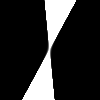
\includegraphics[width=.9\linewidth]{images/GaussianRay1.png}
          \caption{Negative Determinant ellipsoid}
          \label{fig:hyperbolicsub1}
        \end{subfigure}%
        \begin{subfigure}{.33\textwidth}
          \centering
          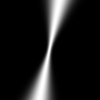
\includegraphics[width=.9\linewidth]{images/GaussianRay3.png}
          \caption{Normalised Major Axis Density}
          \label{fig:hyperbolicsub2}
        \end{subfigure}
        \begin{subfigure}{.33\textwidth}
          \centering
          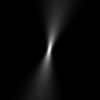
\includegraphics[width=.9\linewidth]{images/GaussianRay2.png}
          \caption{Normalised Cross Section Integral}
          \label{fig:hyperbolicsub3}
        \end{subfigure}
        \caption{A Hyperbolic Distribution with Normalisations}
        \label{fig:hyperbolic}
        \end{figure}
        With a single image from a camera, the only information collected about the location of an object is that it lies somewhere within a narrow cone of infinite length.  (Ignoring exploitable imperfections in the camera such as focal length)
        In the case of stereo imaging, the hyperbolic measurements of points in the near field would immediately reduce to localised ellipsoids, while points in the far field would become narrow hyperbolic distributions.

        The hyperbolic structure is symmetrical like the ellipse, which suggests probability behind the camera.  With decent image classifiers this is unlikely to be a problem as the final localised object will fall on the intersection of the rays.

      \subsubsubsection{Allocating Observations to Objects}
        If multiple observations are made of multiple similar objects, the observations must be allocated to the appropriate object.

        The observations must be ranked by some metric, and sorted.  For \(m\) objects, and \(n\) observations, this takes \(m \times n\) memory.  In our low resolution computer vision pipeline, the number of possible visually non-unique objects is very small, so this product remains quite small in practice.

        The choice of ranking metric is very much a context-dependent decision.  In general though, because the ellipsoids can be interpreted as probability density functions of prediction, there is a function that defines the probability of intersection. The Bhattacharyya distance is a metric used in estimating the separability of clustered data, and makes for a reasonable first-choice of metric.


  \subsection{Results and Discussion}

    \subsubsection{Simulation tests}
      We used the simulator built alongside the arducopter firmware to run our tests.  This simulator is detailed enough to handle the inertial model of the platform and inject noise into the sensors.
      This simulator allows us to run our full software stack on any computer with a functioning compiler.
      The object tracking code estimates the location of the objects using data from the camera and flight controller covering the gimbal pose, the roll, pitch and yaw of the copter, and the GPS location as fused with the accelerometer and gyro data.

      Because the the camera cannot resolve range, an assumption model describing the ground was added to the code reducing the columnar vision model to a spot on the ground.

      Using a servo driven gimbal on the real copter we cannot perform mechanical compensation of the pitch and roll without injecting extremely large angular uncertainties.
      The object estimation code compensates for the pitch and roll using matrices representing body rotations under OpenCV.
      This compensation is designed to cleanly counter the non-linear second order signal injection, but with the camera mechanically coupled to a laptop instead of the simulated copter, the loop becomes completely unstable.

      Commenting out the pitch and roll decoupling code makes the copter very well-behaved in the simulator.  Using a pose generator that attempts to place the object at a ray cast forward and down from the copter, the copter can be confidently led around the simulation environment.  If the object appears behind the copter, the copter moves forward, away from the object, turning around as it does so.

    \subsubsection{Live tests}
      The copter was able to physically follow one object, while tracking multiple others.  Unfortunately, problems in maintaining calibration on multiple systems, particularly the camera gimbal, severely limited the opportunities for testing edge cases in an end-to-end system.

      \subsubsubsection{Navigation System}
        The change from RC inputs to Velocity vector commands for the sake of control linearity resulted in much more predictable and consistent behaviour without significant loss of control bandwidth.
        To reduce the length of the feedback loop, we used the guided waypoint functions and absolute yaw commands in Arducopter 3.2 onward.  This change drastically improved the flight stability of the copter, but significantly reduced the control bandwidth.  The waypoint updates appeared to be obeyed at several Hertz, despite a new request being sent every frame (30Hz).
        The behaviour of our final navigation system was refreshingly predictable and by far the best choice for future development despite the loss of bandwidth.
      
      \subsubsubsection{Object Localisation}
        The observation allocation routine selects the most likely object an observation could refer to. If the associated probability is below some threshold, it instead creates a new object.
        In one of the tests, velocity predictions were enabled along with object creation with an inverted axis on the inertial compensation matrices. This system quickly generated more than seventy unique objects in memory and ran velocity prediction on all of them live. The algorithm's CPU usage never approached the requirements for the computer vision despite running an unoptimised sorting and allocation routine, and uncertainty analysis.
%XXX make all testing past tense
      \subsubsubsection{Object detection}
        %Basic colour matching limitations, false positives
        The feature detection algorithm used in all testing of this platform was very simple colour space thresholding.  In uncontrolled environments, this resulted in multiple detected features with no effective means of differentiating them.  The uncertainty analysis did appear to help with this in the limited live testing it received, but the code was not sufficiently ready to draw any generalised conclusions.

        Many more advanced object detection processes became available on our platform over the course of the project thanks to the work of Tan \cite{Tan}, but these were in active development throughout the project and offered no consistent foundation to test upon.

      \subsubsubsection{Bench Marks}
        As mentioned earlier, the Arducopter firmwares offer a GPS driven ``follow me'' mode using the Android application ``Tower'' \cite{3dr-tower}.
        The GPS tether mode was very stable and eminently usable in real circumstances.  It suffered from worse update bandwidth issues than our autonomous modes, and frequently allowed the beacon to leave the frame.  We can presume that the commodity chase-cams soon to be released will optimise for bandwidth and pay more attention to camera direction.

        The GPS chase system did have some serious flaws though.  In the very poor GPS environment of the Great Court on the UWA campus, the Ublox Neo7m radio was deviating more than 500m every couple of seconds.  With no operator assistance, the loss of GPS led to a catastrophic failure of the algorithm and a very difficult operator intervention.  Fortunately, the Ardupilot firmware permits multiple GPS modules in redundant fashion.  So we were able to combat the urban canyon environment with radio diversity.

\section{Conclusions}

We reviewed, re-designed and re-built the UWA autonomous hexacopter; thereby greatly improving its overall capabilities and making it fit-for-purpose as a development platform for autonomous navigational routines. The re-build involved replacement of both the flight controller and the server. The new flight controller provided the following capabilities:
\begin{itemize}
  \item New gimbal features for the object tracker.
  \item Waypoint navigation.
  \item Robust and consistent failsafe behaviours.
  \item Extended Kalman Filter for flight dynamics.
  \item Live telemetry and reporting of flight parameters.
  %more here
\end{itemize}

During the project, the flight controller firmware advanced from Arducopter V3.2, through V3.3rc10, to V3.3 stable near the end of the project.
The enhanced server supported advanced computer vision routines.
We brought the code-base up to a level where it is feasible to implement rudimentary SLAM processes. We also demonstrated that low-power single board computers can perform live computer vision processes and elements of SLAM processes with uncertainty based reasoning to track and follow moving objects. Our Computer-Vision-Only routines are by no means as robust as radio links and differential GPS, but the use of Computer Vision allows aesthetic framing of more than a wrist-worn GPS beacon. Our Object tracker was demonstrated with a variety of navigation loops, some of which were not GPS dependent. In commodity chase-cams, these control schemes could allow a graceful handover from radio beacon to computer vision in the event of a GPS failure.

%BUSHIT STATEMENT ABOUT YOUR GIFT TO HUMANITY AND THE BRIGHT FUTURE IT UNVEILS.



\section{Recommendations}

  The UWA hexacopter platform is reaching a level of hardware maturity where future work can focus on new algorithms and applications.  Key areas for improvement mainly relate to the gimbal and camera.

  The gimbal can removed entirely in favour of a fixed camera mount, or replaced by a Brushless DC motor driven gimbal for accurate mechanical image stabilisation.  The camera could benefit from a wider angle lens, although the narrow field of view did prompt us to find a sound solution for tracking an object beyond the frame boundary.

  As discussed in section \ref{sec:hyperbolicCase}, the uncertainty analyses are incomplete.
  Without solutions to the hyperbolic uncertainty case or rotational transforms, the object tracker will have somewhat unpredictable accuracy.  However, the system does function and can still benefit from case-specific functions to generate camera angles to suit artistic direction.

  Further exploration of the hyperbolic case and singular matrices would permit the use of Kalman style path prediction and improve the tracking stability.
  Using a vector difference of positions to estimate the velocity, models of objects can be evolved over time and updated with additional measurements.  With additional statistical analysis, this landmark velocity can be extended to a form consistent with a Kalman style motion filter for the each visible landmark.

  % SIFT algorithm
  A problem addressed in section \ref{sec:objectAllocation} is that the objects detected by colour thresholding have a non-zero size which goes against the assumptions implicit in the statistical treatment of the observations.  An algorithm like SIFT would track multiple points on any given object, and provide nearly unique visual identifiers for allocating observations to individual objects.  While this would eliminate a small sorting routine in the object allocator, the overheads of SIFT may well require a larger computing budget.

  %Optical Flow
  Optical Flow is an extremely interesting avenue of research for small UAVs because the high compute-cost can be handled by dedicated silicon like an FPGA.  Coupled with a covariance uncertainty analysis, Optical flow was able to resolve the relationship between relative velocity and proximity between copter and object with every frame from the camera.  
  
  As it stands, the uncertainty analysis in our implementation does not account for correlations between velocity and position, but the matrices can simply be expanded to \(6\times6\) inverse correlation matrices instead of storing independent \(3\times3\) matrices for position and velocity.  The \(6\times6\) matrix also allows the observation-to-object allocator to use velocity as a distinguishing feature when only a correlation between \(\dot{x}\) and \(z\) is known.  For sensors that cannot resolve velocity, the additional matrix elements are just zeroes.
    %XXX See control system theory, state vectors and time-step matrices.

  %Adding a stereo pair of cameras to the copter using the large 550mm base-line afforded by the frame, would create multiple simultaneous position and velocity measurements, eliminating the Z-axis ambiguity over a significant usable range.  
  %Using data from stereo image sources is well solved by our existing uncertainty analysis, though the camera input options are limited on the RPi. I would strongly recommend the inclusion of a vision co-processor to handle frame synchronisation and image mixing if Stereo imaging is explored.  This vision co-processor could also accelerate edge-detection and optical flow processes.

  %Use ROS
  The current structure of the code base is sound, but makes it difficult to run processes like object tracking and object avoidance simultaneously.  This situation could be improved by using a subscriber model between different processes, such as that used by ROS.




  \pagebreak


%Referencing
%---------------------------------------------------------
%\pagebreak
\renewcommand{\refname}{References}
\addcontentsline{toc}{section}{References}
\bibliography{references/refs}
\bibliographystyle{ieeetr}
%\addbibresource{references/refs.bib}
%\printbibliography

%---------------------------------------------------------

\begin{appendices}
  %\addcontentsline{toc}{section}{Appendices}
%  \section{ArduPilot (Pixhawk) Proposal} \label{sec:PihawkProposal}
%    \includepdf[pages=-]{../picopter/Documents2015/ardupilot-proposal/ardupilot-proposal.pdf}


  \section{Atomic Graph-Traversal SLAM Proposal} \label{sec:SLAMproposal}
    
    Storing a motion history of the objects would facilitate the generation of a time-dependent network of estimated locations and relative measurements.
    Here, the nodes represent the instantaneous locations of the objects, linked forward in time by velocity estimates, and linked in space by relative distance measurements.  Assumptions can be added to this mix in the same form as the object locations, time evolution, and relative measurements.

    Building a single covariance matrix for the entire state-space generates extremely large matrices very quickly, and every algorithm that implements full-state covariance pays attention to pruning the map in some way\cite{monoslam} \cite{airshipSLAM}.
    
    A live process need only deal with the instantaneous positions of the robot and a small collection of landmarks. This sub-set of landmarks can be dealt with in a full-state covariance matrix \cite{monoslam}.  
    
    The lesser ``full-state'' covariance matrix can be generated by collapsing dependent chains of observations down using the vector sum, and combining network loops with the intersection into landmarks.  The ``full state'' covariance matrix can be chosen from the resulting landmarks that best reduce absolute navigation uncertainty.  Further observations are still generated as atomic structures and added to the network, then used to refine the larger covariance matrix by the graph traversal algorithm.  

    but the landmark uncertainties can be further refined by a less-than-live by a graph traversal \cite{SLAMgraph}.

    %A SLAM process can be initialised by an assumption in the form of an artificial survey marker at boot. The assumptions can be later removed and replaced by real survey markers, with the map fully regenerated by the graph traversal process which need not be on-board the robot.



\end{appendices}

  
\end{document}


